\section{Evaluation}
\label{sec:evaluation}

\subsection{Experimental Setup}
\label{sec:evaluation.setup}

We implemented our dataflow-guided monitoring architecture by
modifying the ARM version of the gem5 simulator \cite{gem5} to support parallel
run-time monitoring. We model the main and monitoring cores as running at 2.5
GHz with 4-way set-associative private L1 I/D caches and a shared 8-way 2 MB L2
cache. This setup is similar to the Snapdragon 801 processor commonly found in
mobile systems. The dataflow engine uses a 1 kB cache for flags.

In order to explore the generality of the architecture for
different monitors, we implemented four different monitors: uninitialized
memory check (UMC), array bounds check (BC), dynamic information flow
tracking (DIFT), and instruction-mix profiling (IMP).  Uninitialized memory
check seeks to detect loading from
memory locations that are not initialized first. Array bounds check, as
mentioned in Section~\ref{sec:monitoring}, is a monitoring scheme that aims to
detect buffer overflows where memory accesses go beyond the boundaries of an
array. We modify the implementation of {\tt malloc} to set base and bound
metadata information. Dynamic information flow tracking is a security
monitoring scheme
which detects when information from untrusted sources is used to affect the
program control flow (i.e., indirect control instructions). For the benchmarks we consider, we mark data read from
files as untrusted. We implemented a multi-bit DIFT scheme which marks
untrusted data with a 32-bit metadata identifier so
that if an error is detected, it is possible to have information about where
the data originated from. Instruction-mix profiling counts the number of ALU,
load, store, and control instructions that are executed. This profiling
information can be useful for performing optimizations. Additionally, recent
work has shown that this information can be used to detect malicious software \cite{tang-raid14}.

\ED{We need to point out that these monitors cannot be implemented with a simple
1-bit dataflow engine (DIFT) that we use for filtering. 
Point: address potential reviewer questions on why don't we just use a 
programmable dataflow engine for monitoring.}

We tested our system using all C benchmarks from SPECint
CPU2006 \cite{spec2006}. Since our implementation of BC depends on the
modification of {\tt malloc} to set array bounds information, we focus on the C
SPECint benchmarks. Although we do not
show results for the C++ benchmarks, we note that the results for UMC, DIFT, and IMP
for these benchmarks are similar to the other results shown. For each
benchmark, we simulated for 2 billion instructions. An initial slack of 2
million cycles, which is less than 1\% of
the total execution time, is given for a 10\% target overhead. This initial
slack is scaled proportionally for other overhead targets. Unless otherwise
specified, an unrestricted, slack-based dropping policy is used.

\subsection{Baseline Monitoring Overheads}

% Full monitoring overheads
\begin{figure}
  \begin{center}
    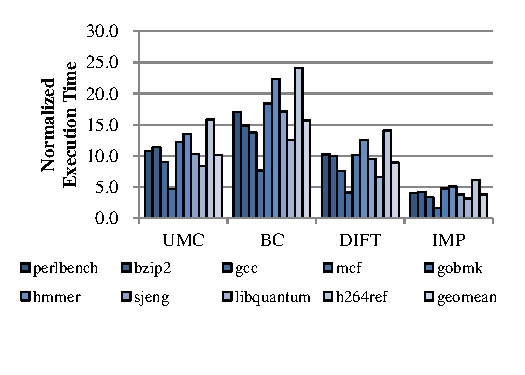
\includegraphics[width=\columnwidth]{figs/data_full_mon.pdf}
    \vspace{-0.2in}
    \caption{Full monitoring overheads for UMC, BC, DIFT, and IMP.}
    \label{fig:evaluation.full_mon}
    \vspace{-0.1in}
  \end{center}
\end{figure} 

Figure~\ref{fig:evaluation.full_mon} shows the execution times of
performing full monitoring normalized to the execution times of the benchmarks
without monitoring. In these results, no filtering or partial monitoring is
done. UMC shows normalized execution times from 5x to 16x with an average
of 10x. BC shows normalized execution times of 8-24x with an average of
16x while DIFT shows normalized execution times of 4x-14x with an average of
9x. IMP shows normalized execution times from 2-6x with an average of 4x. 
These monitors show high overheads because they require several
instructions to process each monitored instruction from the main core. Even
small increases in the number of instructions needed by the monitor lead to
high overheads when multiplied across the main program's execution. For
example, because of the large metadata requirements of UMC, BC, and DIFT, these
monitors must dynamically allocate memory for new metadata. On the other hand,
IMP does not require this dynamic allocation and is overall a simple monitor.
Thus, its overheads are much lower.

\ED{we need to better justify the high overhead. 
Key points: 1) the overhead is in line with LBA, which represent multi-core
monitoring w/ low HW costs.
2) If we are going to mention dynamic memory allocation. We need to say why
it's really necessary -- it's not our implementation problem. It's something
that you need to have for large meta-data. Also, I don't think UMC would need
dynamic allocation.}

\subsection{Filtering of Monitoring Events}

% Full monitoring overheads
\begin{figure}
  \begin{center}
    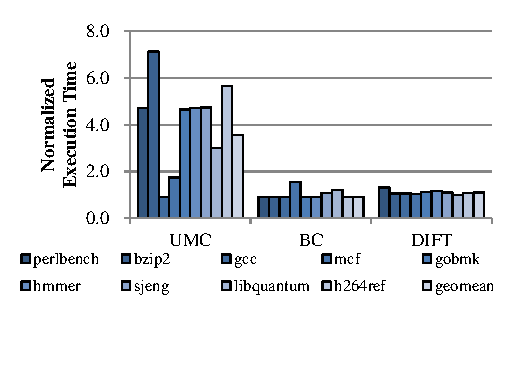
\includegraphics[width=\columnwidth]{figs/data_filtering.pdf}
    \vspace{-0.2in}
    \caption{Monitoring overheads with filtering null metadata for UMC, BC, and DIFT.}
    \label{fig:evaluation.filtering}
    \vspace{-0.1in}
  \end{center}
\end{figure}

Figure~\ref{fig:evaluation.filtering} shows the
normalized execution times with filtering enabled. We see significant
reductions in overhead for all three monitoring schemes. UMC sees normalized
execution times of 1.7-7x with an average of 4x with null metadata filtering.
This is an average reduction in overheads of 65\%. For BC, normalized execution
times drop from 16x down to FIXMEx on average (an FIXME\% reduction). The range of normalized execution
times for filtered BC is FIXME-FIXMEx. This is not surprising since in the baseline
implementation all loads and stores needed to be monitored. However, with
filtering, only loads and stores corresponding to arrays need to be forwarded.
Finally, DIFT sees the largest reduction in overheads with only 10\% overheads
on average after filtering, an 88\% reduction in monitoring overheads, with a
maximum overhead of 31\% after filtering. This is due, in part, to the fact
that
for our implementation of DIFT on SPEC
benchmarks, we only mark data read from files as tainted. For most of these
benchmarks, this propagates to relatively few instructions. Instead, if we
targeted network or streaming applications, which have larger amounts of
untrusted input data, we would expect to see less filtering. IMP does not have
null metadata and thus is not affected by null metadata filtering.

\subsection{Coverage with Adjustable Partial Monitoring}

% BC sweep
\begin{figure*}
  \begin{center}
    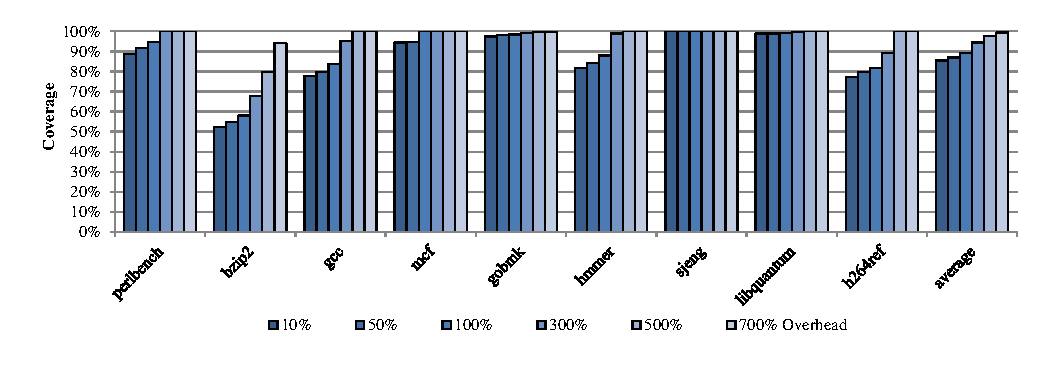
\includegraphics[width=\linewidth]{figs/data_bc_sweep.pdf}
    \vspace{-0.2in}
    \caption{Coverage versus varying overhead budget for array bounds check.}
    \label{fig:evaluation.bc_sweep}
    \vspace{-0.2in}
  \end{center}
\end{figure*}

% UMC sweep
\begin{figure*}
  \begin{center}
    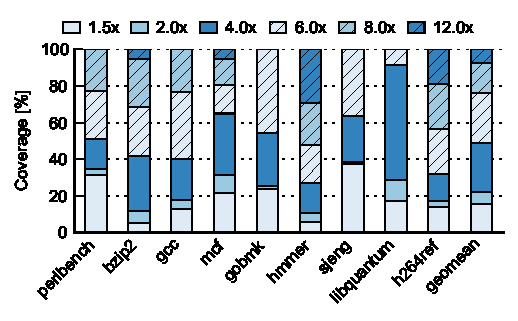
\includegraphics[width=\linewidth]{figs/data_umc_sweep.pdf}
    \vspace{-0.2in}
    \caption{Coverage versus varying overhead budget for uninitialized memory check.}
    \label{fig:evaluation.umc_sweep}
    \vspace{-0.1in}
  \end{center}
\end{figure*}

% IMP sweep
\begin{figure*}
  \begin{center}
    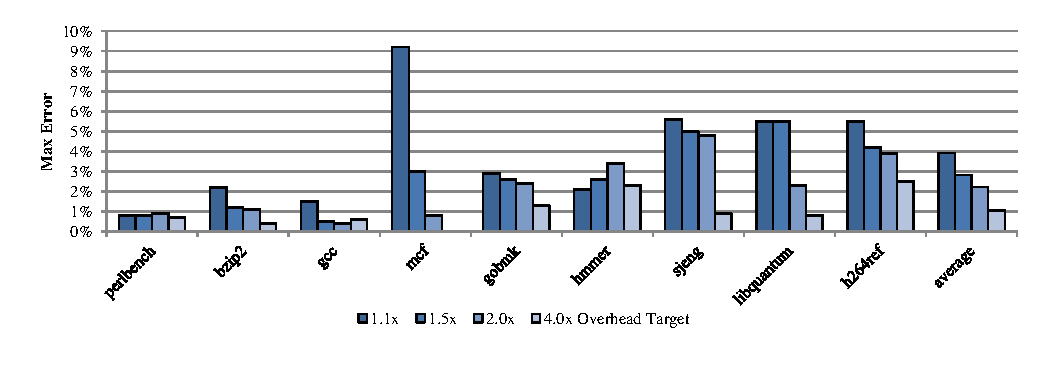
\includegraphics[width=\linewidth]{figs/data_imp_sweep.pdf}
    \vspace{-0.2in}
    \caption{Error versus varying overhead budget for instruction-mix profiling.}
    \label{fig:evaluation.imp_sweep}
    \vspace{-0.1in}
  \end{center}
\end{figure*}

Although the overheads of DIFT are quite low after filtering, BC and UMC still
show significant overheads. Similarly, the overheads of IMP are not improved by filtering. In this section, we evaluate the effectiveness of
using partial monitoring (in addition to filtering) to trade-off coverage for further reduced overheads.
Figure~\ref{fig:evaluation.bc_sweep} shows the monitoring coverage achieved by
array bounds check as we vary the overhead budget. 
We define \emph{monitoring coverage} as the 
percentage of dynamic checks that are performed 
(indirect jumps in DIFT, loads in UMC, and memory accesses in BC). 
The metric is chosen to understand
how likely an error/attack instance is to be detected on an individual system, 
assuming that errors/attacks are uniformly distributed across checks. 
%While we could not evaluate real errors/attacks due to difficulty in setting up
%a large number of bugs and exploits, we believe that the percentage of checks
%provides a good estimate of detection probability when errors/attacks are 
%uniformly distributed across checks.
Note that this metric is different from the
percentage of monitoring events that are not dropped, which includes
non-check instructions.

We see that by varying the overhead budget, the coverage achieved also varies.
With only a 10\% overhead budget, array bounds check still
achieves 82\% monitoring coverage on average. The high coverage
achieved with such low overheads is due to two main effects.  The first is that
monitoring can be done in parallel, providing monitoring coverage without
introducing overheads. The second effect is that, although we aggressively
filter out monitoring events, there may still exist a large number of
monitoring events that do not lead to security or reliability checks. As a
result, dropping these events can reduce overheads without a large impact on
monitoring coverage.

Figure~\ref{fig:evaluation.umc_sweep} shows the analogous graph for UMC. Again
we see that varying overhead budgets enables partial monitoring. We see that
with a 10\% overhead budget, UMC achieves 30\% monitoring coverage on average.
By increasing this overhead budget to 50\%, UMC achieves 48\% coverage. Even
higher coverage can be achieved by allowing higher overheads.

The instruction-mix profiling monitor does not perform check operations. Thus,
the concept of coverage is not applicable here. Instead, for each instruction
type profiled, we calculate its count as a percentage of the total instructions
monitored. We compare these percentages against the case when full monitoring
is performed. Figure~\ref{fig:evaluation.imp_sweep} shows the max error across
instruction types for each benchmark and for varying overheads. We see that
with a 10\% overhead a max error of 9\% is observed and an average of less than
4\%. This error decreases as overhead is increased.

% Flex UMC sweep
\begin{figure*}
  \begin{center}
    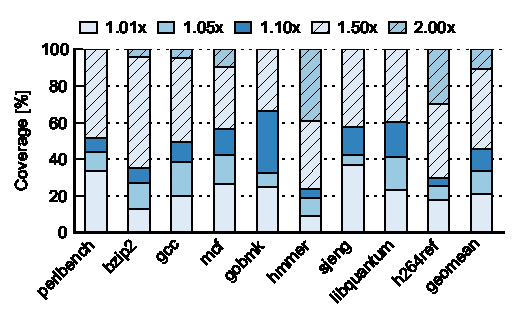
\includegraphics[width=\linewidth]{figs/data_fpga_umc_sweep.pdf}
    \vspace{-0.2in}
    \caption{Coverage versus varying overhead budget for UMC running on an FPGA-based monitor.}
    \label{fig:evaluation.fpga_umc_sweep}
    \vspace{-0.1in}
  \end{center}
\end{figure*}

In addition to evaluating our system for a core-based monitor, we also
evaluated partial monitoring on a higher performance FPGA-based monitor. This
setup is based on the FlexCore \cite{flexcore-micro10} setup and uses a
fully-pipelined monitor running on an FPGA fabric at half the frequency of the
main core. We show results only for UMC. In this case, full overheads of
monitoring range from 10-70\%. Figure~\ref{fig:evaluation.fpga_umc_sweep} shows
the coverage achieved as we sweep overhead from 1-70\%. We see that partial
monitoring can allow the overheads of such a system to be pushed below 10\%
while still providing partial coverage.

\subsection{Comparing Dropping Policies}

% UMC exec time
\begin{figure}
  \begin{center}
    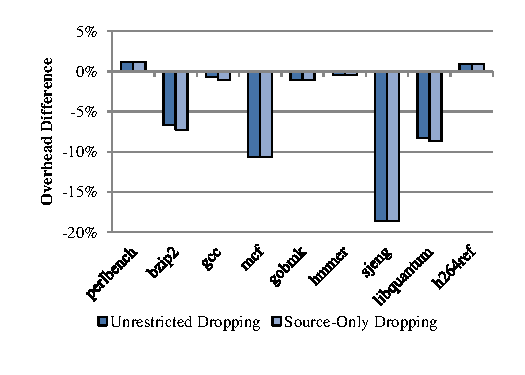
\includegraphics[width=\columnwidth]{figs/data_umc_exec_time.pdf}
    \vspace{-0.2in}
    \caption{Error in meeting overhead budget for uninitialized memory check for different dropping policies.}
    \label{fig:evaluation.umc_exec_time}
    \vspace{-0.2in}
  \end{center}
\end{figure}

% UMC coverage across policies
\begin{figure}
  \begin{center}
    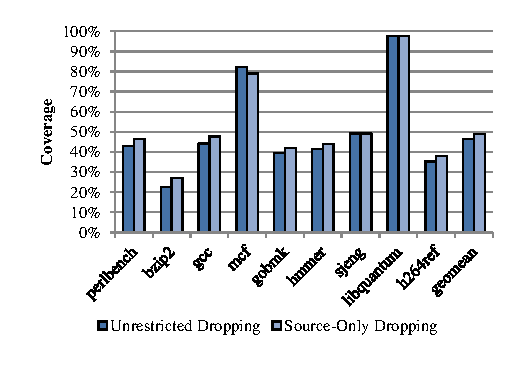
\includegraphics[width=\columnwidth]{figs/data_umc_coverage.pdf}
    \vspace{-0.2in}
    \caption{Coverage for uninitialized memory check for different dropping policies.}
    \label{fig:evaluation.umc_coverage}
    \vspace{-0.1in}
  \end{center}
\end{figure}
In this section we evaluate the trade-offs between unrestricted dropping and source-only dropping.
Figure~\ref{fig:evaluation.umc_exec_time} shows the difference between the
overhead budget and the run-time monitoring overheads for UMC. A positive value
means that the overhead target was overshot while a negative value indicates
that the overhead budget was met. We see similar results for unrestricted
dropping and source-only dropping due to the fact that UMC consists of a large
number of independent monitoring flows.
Figure~\ref{fig:evaluation.umc_coverage} shows the coverage of UMC for
unrestricted dropping and source-only dropping. We see that source-dropping
consistently achieves higher coverage than unrestricted dropping. This is due
to the fact that some of the overheads of monitoring for unrestricted dropping
are being spent on wasted work as discussed in Section~\ref{sec:policies.which}.

% BC exec time
\begin{figure}
  \begin{center}
    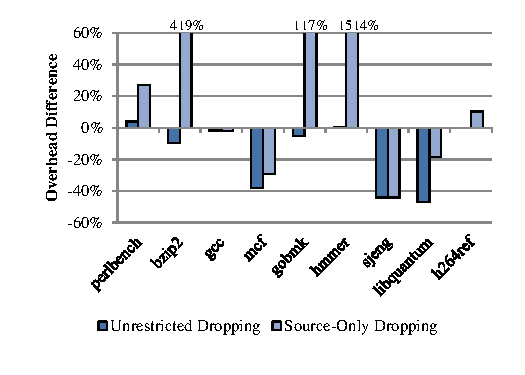
\includegraphics[width=\columnwidth]{figs/data_bc_exec_time.pdf}
    \vspace{-0.2in}
    \caption{Error in meeting overhead budget for array bounds check for different dropping policies.}
    \label{fig:evaluation.bc_exec_time}
    \vspace{-0.2in}
  \end{center}
\end{figure}

% BC coverage across policies
\begin{figure}
  \begin{center}
    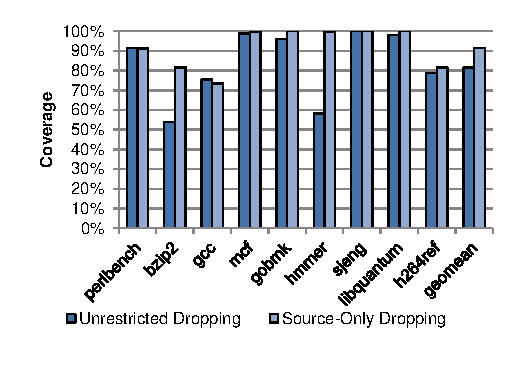
\includegraphics[width=\columnwidth]{figs/data_bc_coverage.pdf}
    \vspace{-0.2in}
    \caption{Coverage for array bounds check for different dropping policies.}
    \label{fig:evaluation.bc_coverage}
    \vspace{-0.2in}
  \end{center}
\end{figure}

Next, we evaluate these trade-offs between source-only dropping and unrestricted dropping for BC.
Figure~\ref{fig:evaluation.bc_exec_time} shows the overhead differences for BC
and Figure~\ref{fig:evaluation.bc_coverage} shows the coverage for BC.
From Figure~\ref{fig:evaluation.bc_exec_time}, we see that for several
benchmarks, source-only drop fails to meet the specified overhead target.
The overshoot of the overhead target is quite high with an overhead difference
of 420\% for {\tt bzip2}, 120\% for {\tt gcc}, and 1500\% for {\tt hmmer}.
Since only array allocations are considered source events for BC, it is
difficult for source-only dropping to match overhead targets. Although
Figure~\ref{fig:evaluation.bc_coverage} again shows higher coverage for
source-only dropping, this is in part due to the fact that is running with
higher overheads.

\subsection{Multiple-Run Coverage}

% Multi-run coverage with unrestricted dropping
\begin{figure}
  \begin{center}
    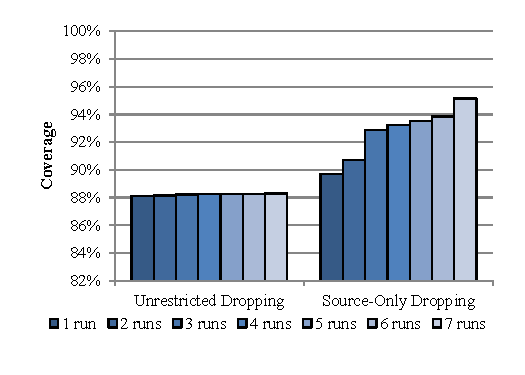
\includegraphics[width=\columnwidth]{figs/data_multirun_coverage.pdf}
    \vspace{-0.2in}
    \caption{Coverage over multiple runs for BC with a 10\% probability to not drop events.}
    \label{fig:evaluation.multirun}
    \vspace{-0.1in}
  \end{center}
\end{figure}

One possible application of partial monitoring with low overheads is to enable
cooperative debugging. 
The idea with cooperative debugging is to use partial
monitoring with very low overheads across a large number of users or runs. By
varying the pattern of partial monitoring done on each run, the goal is to
achieve high coverage across multiple runs. Varying the monitoring that is
done for different runs can be achieved by using a probabilistic dropping policy.
Figure~\ref{fig:evaluation.multirun} shows the total
coverage achieved over multiple runs for array bounds check running for
unrestricted and source-only dropping policies with probabilistic dropping. Here, we use a 10\% probability
that events are not dropped. Since the goal is code coverage, coverage here is
measured as the percentage of static instructions which are monitored. Each run
was simulated for 200 million instructions. 
We see that for the unrestricted dropping policy there is almost no increase in
coverage.  This is due to the fact that since there are multiple dependent
monitoring operations that must be done in order for a final check to be
successful as discussed in Section~\ref{sec:policies.when}.
Instead, source-only
dropping is much better suited for achieving high coverage over multiple runs.
Source-only dropping shows a 5\% increase in coverage with only seven runs.
Over hundreds or thousands of runs, source-only dropping should be able to
reach 100\% code coverage.

\subsection{Area and Power Overheads}

% Area and Power Overheads
\begin{table}[tb]
  \begin{center}
    \vspace{-0.0in}
    \begin{footnotesize}
    
% Full monitoring at zero slack

\begin{tabular}{|c|c|c|}
\hline

{\bf Monitor} & {\bf Peak Power [mW]} & {\bf Runtime Power [mW]} \\ \hline\hline

UMC  & 4.7 (4.9\%) &  3.1 (8.2\%) \\ \hline
BC   & 6.9 (7.1\%) &  4.1 (10.7\%) \\ \hline
DIFT & 7.2 (7.4\%) &  4.3 (11.1\%) \\ \hline

\end{tabular}

    \end{footnotesize}
    \caption{Average power overhead for dropping hardware at a 50\% overhead
    budget. Percentages in parentheses are normalized to the main core
    power.}
    \vspace{-0.2in}
    \label{tab:evaluation.area_power}
  \end{center}
\end{table}

Adding the dataflow engine in order to enable filtering and partial monitoring adds
overheads in terms of area and power. We use McPat \cite{mcpat-micro09} to get
a first-order estimate of these area and power overheads in a 40 nm technology
node. McPat estimates the main core area as 2.71 mm$^2$ and the peak power usage as
965 mW averaged across all benchmarks. The average runtime power usage was 385 
mW. These area and power numbers consist of the core and
L1 cache, but do not include L2 cache, memory controller, and other
peripherals. The power numbers include dynamic as well as static (leakage)
power. For the dataflow engine, we modeled the ALUs used for address
calculation, the dataflow flag register file and cache, the configuration
tables, and the filter decision table. These were modeled using the
corresponding memory and ALU objects in McPat. We
note that this is only a rough area and power estimate since components such as the
wires connecting these modules have not been modeled. However, this gives a
sense of the order-of-magnitude overheads involved with implementing our
approach.

Our results show that an additional 0.197 mm$^2$ of silicon area is needed, an
increase of 7\% of the main core area. Table~\ref{tab:evaluation.area_power}
shows the peak and runtime power overheads averaged across all benchmarks with
a 50\% monitoring overhead target. The peak power is 41-72 mW, which is
less than 8\% of the main core's peak power usage. Similarly, the average runtime power is 20-43
mW, corresponding to 5-11\% of the main core's runtime power.

